\documentclass[TAU.tex]{subfiles}
\begin{document}

\chapter{Основные понятия, структура и классификация систем автоматического управления}

 С древних времен человек хотел использовать предметы и силы природы в своих целях, то есть управлять ими. Теория управления пытается ответить на вопрос «как нужно управлять?». До XIX века науки об управлении не существовало, хотя первые системы автоматического управления уже были (например, ветряные мельницы «научили» разворачиваться навстречу ветру). Развитие теории управления началось в период промышленной революции. Сначала это направление в науке разрабатывалось механиками для решения задач регулирования, то есть поддержания заданного значения частоты вращения, температуры, давления в технических устройствах (например, в паровых машинах). Отсюда происходит название «теория автоматического регулирования». Позднее выяснилось, что принципы управления можно успешно применять не только в технике, но и в биологии, экономике, общественных науках.

\section {Процессы управления}
%Процессы управления (слайд 3) - понятия, общая информация о процессах + таблица

Процессы управления и обработки информации в системах любой природы изучает наука кибернетика. Один из ее разделов, связанный главным образом с техническими системами, называется теорией автоматического управления. 

\begin{center}
Процессы управления\\ [4pt]
\begin{tabular}{|p{6.5cm}|p{6.5cm}|}
  % after \\: \hline or \cline{col1-col2} \cline{col3-col4} ...
  \hline
  {\Large В живой природе} & {\Large В неживой природе} \\ [4pt]
  \hline
  Естественный отбор & Наведение на цель орудия \\
  \hline
  Терморегуляция у животных & Поддержание температуры в печи\\
  \hline
  Поддержание равновесия животными & Поддержание равновесия робота\\
  \hline
  Увеличение рождаемости в стране & Поддержание скорости на моторе\\
  \hline
  Уничтожение клеток определенного типа (вирусных, инфекционных и т.п.)& Поддержание фиксированной высоты летального аппарата\\
  \hline
  Повышение работоспособности работников предприятия & Поддержание заданного напряжения\\
  \hline
\end{tabular}
\end{center}

\section{Характеристика процессов управления}
%Характеристика процессов управления (слайд 4) - пара слов о каждой характеристике + примеры

Общие характеристики всех процессов управления:
\begin{itemize}
  \item Прием информации - поиск и обнаружение сигналов (выделение сигналов из шума). Примеры: камера, глаз, датчики давления, скорости, положения и т.п., общение.
  \item Хранение информации - процесс поддержания исходной информации в виде, обеспечивающем выдачу данных по запросам конечных пользователей. Примеры: память животных, память на носителях - USB, HDD, CD, DVD.
  \item Преобразование информации - процесс изменения формы представления информации или ее содержания. Примеры: анализ рынка, те или иные вычисления.
  \item Выработка управляющего воздействия - подача напряжения на мотор, передача указаний подчиненным, поворот руля. %-не очень понятно, уточнить.
\end{itemize}

\section{Исходные положения ТАУ}
\subsubsection{САУ. Структурная схема и понятия}
%САУ. Структурная схема и понятия (слайд 5-6) - схема, описание, термины. Что входит в схему, как работает, назначение каждого элемента

\defi{\it Управление} - целенаправленное воздействие не объект или устройство. Управление может быть автоматическим, т.е. без участия человека, ручным, т.е. в присутствии человека, или полуавтоматическим, т.е. работающим при участии человека.

\defi{\it Объект управления} (ОУ) - устройство, которым нужно и можно управлять. Это может быть автомобиль, самолет электродвигатель и т.д.

\defi{\it Цель управления} ОУ - поддержание 
\textit{заданного} 
режима, т. е. изменение какого-либо параметра ОУ по заданному закону (например температура в холодильнике должна быть зафиксированной). Такой параметр называют 
\textit{управляемой} или 
\textit{выходной} переменной. 

\defi{\itСистема автоматического управления} (САУ) - устройство управления (УУ) и объект управления (ОУ).\par
Основной задачей автоматического управления является поддержание определенного закона изменения одной или нескольких физических величин, характеризующих процессы, протекающие в ОУ, без непосредственного участия человека. Эти величины называются {\it управляемыми величинами}. Если в качестве ОУ рассматривается хлебопекарная печь, то управляемой величиной будет температура, которая должна изменяться по заданной программе в соответствии с требованиями технологического процесса. 



\begin{figure}[h]
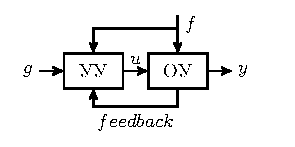
\includegraphics[width=10cm]{SAU_scheme.pdf}
\caption{На структурной схеме САУ: $y$ --- выходная переменная; $g$ --- задающее воздействие (иногда изображается как выход задающего устройства); $f$ --- возмущение, действующее на ОУ и, возможно, на УУ; $u$ --- управление (управляющее воздействие). Канал связи, по которому поступает информация в УУ о состоянии ОУ, называется {\it обратной связью} (feedback). В САУ обратная связь может отсутствовать.}
\centering
\end{figure}

\subsubsection{Понятие устойчивости}
ОУ в зависимости от входных воздействий бывают устойчивые, нейтральные и неустойчивые. Например, пусть при постоянных $u = u_0, f = f_0$ на выходе $y = y_0$. Положим, что на какое-то время $T$ значение $u$ и $f$ изменились, а затем вернулись к исходным значениям. Тогда объект управления

\begin{itemize}
    \item устойчивый, если при $t \rightarrow \infty$ выход $y \rightarrow y_0$; \\
Например, холодильник, генератор напряжения, маятник, унитаз.
    \item нейтральный, если при $t \rightarrow \infty$ выход $y \rightarrow y_1$ и $y_1\neq y_0$. \\
Например, резервуар с водой;
    \item неустойчивый, в противном случае.\\
Самолет с обратной стреловидностью крыла, обратный (перевернутый) маятник.
\end{itemize}

\defi{\it Устойчивость} - это свойство системы возвращаться в установившееся состояние после того, как она была выведена из этого состояния каким-либо возмущением. 
\section{Принципы управления}
В основе построения систем автоматического управления лежат некоторые общие фундаментальные принципы управления, определяющие,каким образом осуществляется увязка алгоритмов управления с заданным и фактическим функционированием, а иногда и с причинами, вызвавшими отклонение.\par
Принято различать три фундаментальных принципа управления: программное управление, принцип компенсации и принцип обратной связи.

\section{АСУ}

\section{Классификация САУ}

\section{Типовые законы управления}
\subsubsection{ПД-закон}

